\xchapter{Metodologia}{}

%O processo de mineração de opinião
%\begin{itemize}

%\item Preprocessing
%\begin{itemize}
%\item Definição
%\item Reiterar o tipo de análise escolhida: Document Level Analysis
%\item Datasets utilizados (Cornell e Amazon - descreve as caracteristicas de cada dataset, como quantidade, balanceamento, natureza, etc.)
%
%\item Descrever e justificar as tarefas envolvidas:
%\begin{itemize}
%\item O texto é dividido em sentenças
%\item POS Tagging - Brill's Tagger
%\item Blocos irrealis são filtrados ou não (atualmente NÃO FILTRAM)
%\item Defino quais ngrams serão extraídos
%\begin{itemize}
%\item Defino o uso do tipo de negação (FAR NEGATION - REFER)
%\item Os verbos foram recentemente removidos do universo
%\item Depois de testar, MANUALMENTE, diferentes configurações de n-grams, mantendo os demais parametros fixos, restaram adjetivos e adverbios, com unigrams, bigrams e trigrams
%\end{itemize}
%
%\item Retorna um vetor de n-grams (bag-of-words)
%\item Resume o subcapitulo e finaliza falando da saída dessa fase para a próxima
%\end{itemize}
%\end{itemize}
%\end{itemize}

\todo[inline]{Falta uma contextualização e uma definição do problema que propomos tratar: determinação da polaridade binária (pos e neg) de documentos, mais especificamente de comentários feitos por usuários sobre itens diversos.E usando features extraídas dos textos buscando uma abordagem mais independente de domínio do que a abordagem baseada diretamente em termos (bag of words)}

Dada nossa proposta de criar e avaliar um sistema fuzzy automatizado de mineração de opinião para classificar o sentimento geral de opiniões encontradas em textos de documentos, o próximo passo foi definir com mais exatidão nosso problema e a tarefa a ser desempenhada. A classificação dos documentos é binária, classificando-os como positivos, que exprimem um sentimento geral positivo sobre um determinado assunto, ou negativos, que exprimem um sentimento geral negativo. E a abordagem de classificação é independente do domínio em que as opiniões são expressas, como cinema, livros ou automóveis. Essa abordagem utiliza características extraídas dos próprios documentos, comuns a documentos de outros domínios, em vez de usar diretamente, por exemplo, os termos existentes nos textos, como realizado em \cite{pang2002thumbs, pang2004sentimental, pang:2008}. Para executarmos nossa tarefa de classificação da polaridade dos documentos, é preciso seguir seis etapas comumente utilizadas em processos de mineração de opinião: a i) definição do domínio, ii) pré-processamento, iii) transformação, iv) seleção de características, v) classificação e vi) análise dos resultados \cite{moraes2012document}. 

\todo[inline]{faça um overview das estapas, descreve resumidamente as etapas para dar uma idéia geral antes de detalhar cada uma}

A etapa de definição do domínio é o momento em que é estabelecido a quantidade e os tipos de domínios que serão utilizados, além de buscar e analisar as bases de dados disponíveis nos trabalhos relacionados ou em outras origens. O pré-processamento é a etapa onde as bases escolhidas são preparadas para serem utilizadas nas próximas etapas, estruturando e filtrando os termos originais dos textos. A transformação é o momento em que os termos estruturados do pré-processamento são transformados em dados numéricos. A etapa de seleção de características envolve uma sub-etapa de extração de características dos dados numéricos. Uma vez extraídas as características, as mais aptas para caracterizar os documentos são selecionadas para serem usadas na etapa seguinte. A etapa de classificação é o onde a base de regras é gerada a partir das regras selecionadas e usada para classificar os documentos. E, por fim, a etapa de avaliação é onde a performance da classificação é avaliada. 

\begin{figure}[h]
\caption{Etapas do processo de mineração de opinião.}
\centering
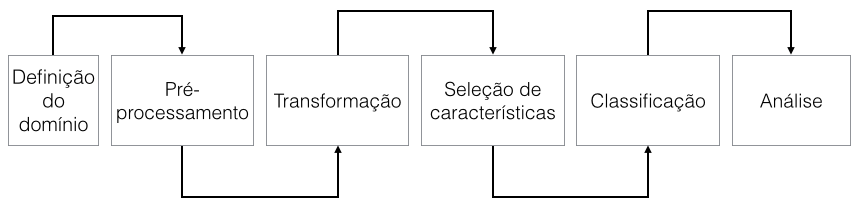
\includegraphics[scale=0.55]{opinion_mining_process_2.png}
\label{figura:processo_mineracao}
\end{figure}

\todo[inline]{ficou muito pequeno o texto dentro das caixas da figura}

\section{Definição do domínio e o pré-processamento dos dados}

\todo[inline]{qual a motivação para escolher vários domínios? contextualize motivando antes de detalhar (já fiz a alteração)} Domínios diversos foram escolhidos para serem analisados por essa pesquisa, dentre eles filmes, livros, carros, computadores, panelas, hotéis, músicas, celulares, mp3, pen-drives, dispositivos gps, wifi e câmeras fotográficas. Essa diversidade de domínios é importante para avaliar nossa proposta em contextos variados, assim como para buscar um classificador menos dependente de domínio. Foram escolhidas bases já conhecidas para avaliação de pesquisas na área, desta forma todas as bases de dados são da língua inglesa.

Para filmes, nós selecionamos a largamente utilizada base de dados \textit{Movie Review Sentiment Polarity Dataset v2.0}\footnote{Disponível em: \url{https://www.cs.cornell.edu/people/pabo/movie-review-data/}. Veja uma lista de trabalhos utilizando esta base em \url{https://www.cs.cornell.edu/people/pabo/movie-review-data/otherexperiments.html}}, desenvolvida e utilizada inicialmente por \cite{pang2004sentimental}. Ela é uma base de dados balanceada, pois tem a mesma quantidade de documentos positivos e negativos. Ela possui 2000 documentos com opiniões sobre filmes, 1000 positivos e 1000 negativos, retirados do site IMDB \footnote{\url{http://www.imdb.com}}. Os documentos foram previamente classificados pelos autores e todos os demais dados originais foram removidos, como data, autor, gênero, assunto, título, dentre outros, restando somente o texto original das opiniões. Os textos ainda foram divididos em sentenças, onde cada linha é uma frase do documento.

As opiniões sobre livros, carros, computadores, panelas, hotéis, músicas, celulares estão reunidos numa base de dados balanceada com 400 documentos \todo[inline]{qual o nome da base? disponível em qual endereço?} produzida por \cite{taboada2011lexicon}, chamada de ``Epinions 1`` \footnote{Disponível em: \url{http://www.sfu.ca/~mtaboada/research/SFU_Review_Corpus.html}}. Os documentos com as opiniões foram extraídas do site Epinions \footnote{\url{http://www.epinions.com/}}, das categorias já citadas. Cada categoria possui 50 documentos, 25 positivos e 25 negativos e eles foram classificados como positivos ou negativos pelos autores através de uma marcação, "recomendado" ou "não recomendado", nos textos opiniativos inseridos pelos próprios usuários. Todos os demais dados originais foram removidos, como data, autor, gênero, assunto, título, dentre outros, restando somente o texto original das opiniões.

E para opiniões de domínios de mp3, pen-drives, dispositivos gps, wifi e câmeras fotográficas, nós utilizamos um recorte balanceado de 2000 documentos de uma base de dados chamada  "Amazon-83713" \footnote{Disponível em: \url{http://patty.isti.cnr.it/~baccianella/reviewdata/index.php?download}}, que contém opiniões sobre os produtos do site da Amazon.com. Parte dessa base já foi utilizada em outros trabalhos como \cite{baccianella2010selecting} e \cite{baccianella2014feature}. Cada documento contém três informações: um identificador único, o texto original e escore, dentro de uma escala de 1 a 5. Este trabalho utilizou o escore para classificar os documentos e serem usados nessa pesquisa. Todos os documentos com escore igual ou menor que 2 foram considerados negativos e com escore igual a 4 ou 5, considerados como positivos. Documentos com escore igual a 3 foram descartados, por não se encaixarem nem em uma classe ou em outra. É importante frisar também que nós fizemos o recorte balanceado de 2000 documentos, pois essa base é originalmente altamente desbalanceada, com muito mais documentos positivos que negativos. \todo[inline]{qual o nome da base? disponível em qual endereço? também cite se houver, o trabalho que desenvolveu ou usou primeiro} 

\todo[inline]{sugiro o termo opinião e não crítica, que me parece algo feito por um especialista}
\todo[inline]{faltou detalhar melhor e caracterizar as bases, de onde vieram os dados? quem são os autores das opiniões?usuários do site? como foram selecionadas as opiniões? qual o tamanho médio, mínimo e máximo? qual o período (mês ou ano) a que se referem? como foram pré-processadas e qual o formato disponibilizado? qual é o conteúdo exatamente das bases? opiniões associadas com uma classe de polaridade? positivo, negativo e neutro? tem outras informações relevantes na base?}

%Existem três níveis básicos de análise de documentos em mineração de opinião: i) nível de análise de documento, ii) sentenças e iii) entidades e seus aspectos. O primeiro nível foca em classificar a opinião geral de um documento expressando-a como positiva ou negativa. O segundo nível, o de sentenças, em vez de considerar o sentimento geral das opiniões presentes em um documento como todo, classifica as opiniões de cada sentença separadamente. E o último nível foca em descobrir todos os alvos existentes nas sentenças do documento, e classifica as opiniões direcionadas a eles \cite{bing:2012}. 
%--------------> Comentei, pois vai para o capitulo 2 <--------------
\todo[inline]{isto deve ser dito no capítulo 2}

Após a definição de um ou mais domínios é preciso, antes de iniciar a etapa de pré-processamento, definir o nível da análise que será feita sobre os documentos. Este trabalho decidiu utilizar o nível de análise de documento por ser o nível mais utilizado entre os trabalhos relacionados, como os trabalhos de \todo[inline]{porque?} \cite{joachims1998text, pang2002thumbs, gamon2004sentiment, mullen2004sentiment, pang2004sentimental, cui2006comparative}. \todo[inline]{porque estas citações? exemplos?}. \todo[inline]{isto é parte da definição do problema, vai para o início do capítulo}

As bases selecionadas devem passar pela etapa de pré-processamento para se adequarem às etapas seguintes. Isto envolveu as tarefas seguintes tarefas:  \todo[inline]{Em nossa proposta, isto envolveu as tarefas de ... (não pode ter este tom geral, ou de exemplificação, é a nossa metodologia, então tem que ser específico}  a tokenização dos documentos, marcação gramatical das palavras (do inglês, \textit{Part of Speech Tagging} ou POST), \sout{filtragem de sentenças com modais} e definição os n-grams que serão utilizados para construir o modelo que represente o documento. \todo[inline]{MATHEUS: retirei a remoção dos modais, pois com a inclusão dos advérbios, a remoção dos modais não ajudou}

A tokenização dos documentos divide o conteúdo de cada documento em sentenças e, por sua vez, em palavras para que o marcador gramatical (ou \textit{tagger}) possa identificar as classes gramaticais das palavras do documento. O marcador gramatical usado foi o proposto \todo[inline]{discutido ou proposto?}  por \citeonline{brill1995transformation} e também usado em trabalhos relacionados a esta pesquisa, como em \cite{chaovalit2005movie, taboada2008extracting, taboada2011lexicon}. O marcador gramatical é um sistema que processa um texto num determinado idioma, identifica e atribui partes de discurso para cada palavra nesse texto, como substantivos, verbos, adjetivos, advérbios, dentre outros \footnote{A lista completa das partes do discurso para o idioma inglês pode ser encontrado em: \url{https://www.ling.upenn.edu/courses/Fall_2003/ling001/penn_treebank_pos.html}}. 
\todo[inline]{descreva um pouco mais o que é um POS tagger (ou faça isso no capítulo 2), e quais as classes gramáticais associadas a cada palavra}

\sout{A tarefa seguinte é a remoção de sentenças que possuem verbos modais \todo[inline]{como foi feito isso?}. Segundo \citeonline{taboada2011lexicon}, modais como "would", "could", dentre outros, presentes numa sentença indicam que as palavras que aparecem juntamente com eles podem não ser confiáveis para serem usadas na definição do sentimento geral de opiniões de um documento.} 

A tarefa final é definir como compor o modelo que representará o documento. O tipo de modelo utilizado nessa pesquisa é o popular saco de palavras (\textit{bag-of-words}), em que cada documento é representado por um vetor de termos (ou n-grams) do documento \cite{moraes2012document}. N-grams são termos que podem ser unigrams (uma palavra), bigrams (duas palavras) ou trigrams (três palavras). 

\todo[inline]{porque 5 tipos? apresente a motivação para nossa escolha} 

Os trabalhos de \cite{hatzivassiloglou2000effects} e \cite{wiebe2000learning} demonstraram que adjetivos são bons indicadores de subjetividade e sentenças opinativas. Contudo, embora adjetivos isolados possam indicar a presença de opiniões, é possível que não haja contexto suficiente para determinar se o sentimento geral das opiniões é positivo ou negativo. Em \cite{chaovalit2005movie} foi reiterado a importância dos adjetivos e adicionou os advérbios como elementos que também provêem subjetividade, enquanto que os demais termos provêem contexto; e \cite{benamara2007sentiment} demonstrou que advérbios são importantes modificadores de intensidade dos adjetivos e influenciam significativamente na determinação do sentimento geral das opiniões de um documento. Dessa forma, nós definimos 5 tipos de n-grams: adjetivos e advérbios como unigrams; advérbios com adjetivos (e.g. \textit{very good}), advérbios com advérbios como bigrams; e a combinação de dois advérbios e um adjetivo como trigram (e.g. \textit{not very nice}) \cite{pang2002thumbs, turney2002thumbs, taboada2008extracting, karamibekr2012verb}. 

Neste processo,também extraímos tipos especiais de bigrams e trigrams: \todo[inline]{justifique porque} n-grams negados (e.g. \textit{not bad}, \textit{nothing special}). Nós aplicamos uma versão simplificada da técnica usada em \cite{das2001yahoo} para detecção de negação. N-grams negados podem tanto inverter a polaridade local de um termo ou sentimento geral de uma frase ou documento, quanto podem intensificar a polaridade geral (e.g. \textit{not only good but amazing}). Além disso, \cite{taboada2008extracting} demonstrou que, embora pequena, o tratamento de negação em mineração de opinião, na média, produz melhores resultados na classificação dos documentos. 

Ao fim do estágio de pré-processamento, cada documento é transformado num vetor de n-grams associado às respectivas partes de discurso (advérbio, adjetivo) de cada termo do verto e é passado para a etapa de transformação.  \todo[inline]{a classe gramatical associada também é passada para etapa seguinte?}

\section{Transformação}

%\item Transformation
%\begin{itemize}
%\item O que é
%\item Uso de dicionários de opinião para transformar n-grams e numeros
%\item Explicar porque o uso de dicionarios de opiniao é bom para nosso trabalho
%\item Sentiwordnet (falar sobre explicar, genericamente, como é criado, como é estruturado, valores associados aos termos)
%\item Falar do trabalho de Guerrine que propoe diferentes formulas para determinar a polaridade de um n-gram. E que são melhores que a mais frequente do SWN
%\item Falar e explicar os intensificadores
%\item Negação
%\item Frequencia de n-grams como transformador da polaridade
%\item Compensação de bias negativo
%\item Resume o subcapitulo e finaliza falando da saida dessa fase para a proxima 
%\end{itemize}

A etapa de transformação produz representações numéricas a partir dos vetores de n-grams da etapa de pré-processamento. Cada n-gram é associado a um valor numérico, um grau de polaridade opinativo, usando um dicionário de opiniões \cite{ballhysa2012fuzzy, moraes2012document, mouthami2013sentiment}. Neste trabalho, o dicionário utilizado foi o SentiWordNet 3.0\footnote{Disponível em: http://sentiwordnet.isti.cnr.it/. Download de 22/01/2013} \cite{baccianella2010sentiwordnet}.

\subsection{SentiWordNet 3.0}

O SentiWordNet 3.0 (SWN) é a terceira versão do SentiWordNet, apresentado por \cite{esuli2006sentiwordnet}. É um dicionário criado pela anotação automática de cada \textit{synset}, conjuntos de sinônimos, do Wordnet 3.0, outro dicionário na língua inglesa \cite{fellbaum2005wordnet}. Cada \textit{synset} $s$ é associado pelo SWN a três  escores numéricos $Pos(s)$, $Neg(s)$ e $Obj(s)$ que indicam o quanto positivos, negativos e "objetivos" (ou neutros) são os termos existentes no \textit{synset} \cite{baccianella2010sentiwordnet}. 

 \todo[inline]{fica difícil de entender o que seriam os synsets, principalmente essa notação com parenteses, acho que um pouco mais de detalhe pode ajudar, coloca também um screenshot ou figura do exemplo. PS: o que seria o J nessa notação de synset?}
 
O método de criação do SWN se baseia num conjunto de classificadores ternários \footnote{Um classificador \textit{n-ário} é um dispositivo que atribui a cada objeto exatamente um rótulo a partir de um conjunto pré-definido de $n$ rótulos.} que são capazes de decidir quando um \textit{synset} é positivo, negativo ou objetivo \cite{esuli2006sentiwordnet}. Cada classificador difere um do outro pelos conjuntos de treinos, produzindo diferentes resultados para os \textit{synsets} do Wordnet. O escore final do \textit{synset} é determinado pela proporção normalizada dos classificadores ternários que conseguiram associar um rótulo ao \textit{synset}. Se todos os classificadores concordarem em associar o mesmo rótulo para um \textit{synset}, aquele rótulo (e.g. positivo) terá escore máximo para aquele \textit{synset}. De outra forma, cada rótulo terá um escore proporcional ao número de classificadores que associaram um rótulo a ele. Por exemplo, 3 classificadores assinalaram positivo para um dado \textit{synset}, um outro classificou o \textit{synset} como negativo, e nenhum conseguiu classifica-lo como objetivo. Assim o \textit{synset} terá $Pos(s) = 0.75$, $Neg(s) = 0.25$ e $Obj(s) = 0$. Como a proporção é normalizada, os valores estão num intervalo $[0,1]$ e a soma dos três escores também sempre será igual a 1. Assim, é possível que existam (e existem) \textit{synsets} que tenham todos os três graus diferentes de zero, indicando que há termos positivos, negativos e objetivos ao mesmo tempo \cite{esuli2006sentiwordnet}. A figura \ref{figura:bad_synset} ilustra o \textit{synset} do termo \textit{bad}.

\begin{figure}[h]
\caption{Exemplo do \textit{synset} do unigram \textit{bad}}
\centering
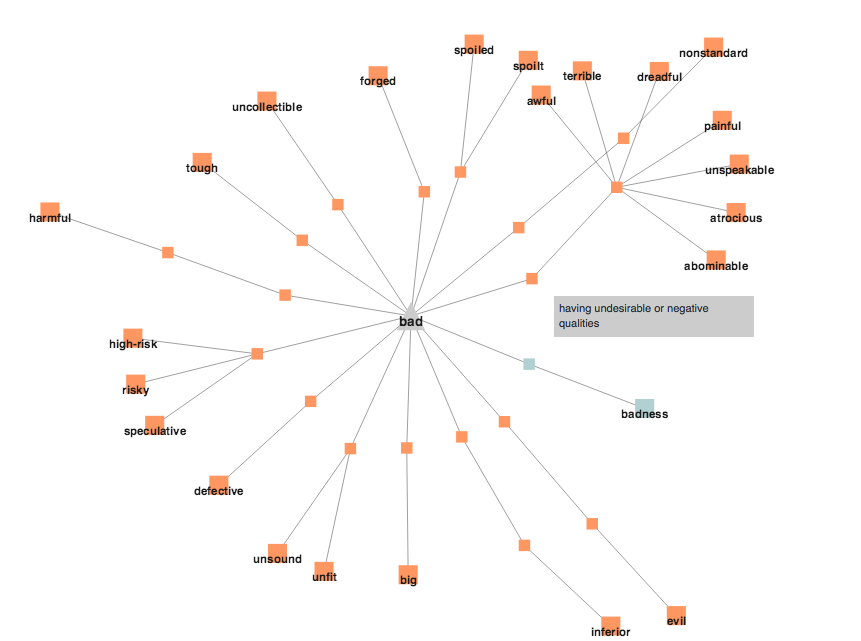
\includegraphics[scale=0.5]{bad_synset}
\label{figura:bad_synset}
\end{figure}
 
A palavra \textit{bad} liga-se aos seus sinônimos através de relações chamadas \textit{glosses} (retângulo em cinza escuro) que são significados que aqueles sinônimos tem num determinado contexto. Na figura, \textit{bad} liga-se a \textit{awful} e \textit{terrible}, por exemplo, através de uma relação em que eles significam ter "indesejada ou qualidade negativa".
 
 \todo[inline]{Falta justificar porque fizemos esse calculo de Pol e não usamos Pos e Neg, começa o parágrafo apresentando a motivação e depois o que fizemos}
 
Para que pudéssemos extrair as características, seleciona-las e, então, principalmente, gerar a base de regras fuzzy nas etapas seguintes, foi preciso simplificar a tupla de três valores dos termos do SWN. Em \cite{ohana2009sentiment} e \cite{khan2011sentiment} a tupla do SWN também foi simplificada para um único valor para determinar a polaridade de cada termo. Inicialmente, nós definimos a polaridade resultante $Pol(n)$ de um termo  $n$, marcado gramaticalmente (e.g. adjetivo, advérbio, etc.), como $Pol(n) = Pos(s) - Neg(s)$ ,subtraindo o grau de positividade do grau de negatividade do \textit{synset} $s$ mais freqüente a que pertence o unigram. Por exemplo, o \textit{synset} mais freqüente de \textit{good} é o próprio \textit{good}, com grau $Pos(s)$ de 0.75, $Neg(s)$ de 0.0 e $Obj(s)$ de 0.25. A polaridade resultante $Pol(n)$ será de 0.5. Contudo, há um problema em escolher um \textit{synset} adequado para uma palavra, uma vez que para um mesmo termo pode haver mais de 1 \textit{synset} associado. No trabalho de \cite{guerini2013sentiment} é demonstrado que escolher o \textit{synset} mais freqüente pode não ser melhor que escolher um qualquer de maneira aleatória. No mesmo trabalho, também são demonstradas outras fórmulas de se calcular a polaridade termos do SWN, chamados pelos autores de palavras fora de contexto (do inglês \textit{word’s prior polarity}). Palavras fora de contexto são típicas de abordagens \textit{bag-of-words} e devem ter um tratamento diferente para se adequar ao problema da perda do contexto causada na etapa de pré-processamento, com a tokenização do documento \cite{guerini2013sentiment}. Assim, nós utilizamos uma das fórmulas de \cite{guerini2013sentiment} para calcular a polaridade $Pol(n)$ de um termo do SentiWordNet. 

\todo[inline]{avaliamos isso e chegamos a essa conclusão? ou estamos admitindo isso a partir de outro trabalho? acho melhor dizer que há um problema de escolher o synset adequado para um termo uma vez que para um mesmo termo pode have mais de 1 synset, e uma abordagem utilizada em alguns trabalhos é escolher o mais frequente, porém outros trabalhos mostraram que isso pode não ser melhor do que escolher um synset aleatoriamente (citacao)}  

\sout{Além disso, o uso de polaridades de palavras fora de contexto (do inglês \textit{word’s prior polarity}), típicas de abordagens \textit{bag-of-words}, deve ter um tratamento diferente para se adequar ao problema da perda do contexto causada na etapa de pré-processamento, com a tokenização do documento  \cite{guerini2013sentiment}. Assim, nós utilizamos um dicionário derivado do SWN produzido por  \cite{guerini2013sentiment} com todas as polaridades fora de contexto calculadas de todos os termos do SentiWordNet 3.0.\todo[inline]{o que é exatamente esse dicionáro derivado? ficou muito rápido a explicação aqui} A polaridade resultante $Pol(n)$ agora é a polaridade fora de contexto do unigram. }

O uso da abordagem de polaridades fora de contexto tem a vantagem de ser mais rápida e simples do que uma profunda análise semântica ou desambiguação (uma linha de pesquisa completa, por si só) para assinalar um valor de polaridade para um termo, além de ser independente de domínio, como proposto nesse trabalho. Além disso, dicionários construídos automaticamente, como o SWN, superam problemas existentes de dicionários criados manualmente, como em \cite{taboada2008extracting, taboada2011lexicon} que tendem a se restringir a um número muito menor de termos, consomem mais tempo para serem construídos e podem sofrer enviesamento de seus autores \cite{ohana2009sentiment}. Outra vantagem de usar técnicas baseadas em dicionários é que dispensa o uso de grandes bases de dados para aprendizado ou motores de buscas com funcionalidades especiais para a tarefa \cite{khan2011sentiment}. A principal desvantagem, todavia, é que a fase de  transformação depende inteiramente da cobertura do dicionário utilizado \cite{khan2011sentiment}. 

\subsection{Definição da polaridade}

\subsubsection{Unigrams}

Dado um unigram do vetor de n-grams de um documento, a polaridade deste é definida pela polaridade do termo fora de contexto provida pelo dicionário de opiniões. Embora somente as formas base das palavras sejam armazenadas no Wordnet e, por conseguinte, no SWN, a grande maioria das buscas são feitas pelas formas flexionadas das palavras oriundas dos documentos. Assim, para podermos definir a polaridade dos unigrams, e dos n-grams seguintes, nós utilizamos o conjunto de funções morfológicas do próprio Wordnet \footnote{Vide \url{https://wordnet.princeton.edu/man/morphy.7WN.html}} para gerar as formas existentes no dicionário a partir formas flexionadas das palavras dos vetores de n-grams. \sout{Caso o unigram não seja encontrado no dicionário, o lema deste é utilizado} \todo[inline]{o que é o lema e como obtem?}. Caso o unigram não seja encontrado no dicionário ele é descartado do processo.

Nós também analisamos a existência de múltiplas ocorrência do mesmo unigram no documento. Por exemplo, no documento:

\textit{Overall, the movie was great. The acting was great, the history was great, and the direction was just plain great.}

A repetição da palavra \textit{great} sugere que a pessoa que escreveu a crítica acima não tinha um termo específico que expressasse outras opiniões e utilizou \textit{great} como um termo positivo geral. Além disso, uma palavra que aparece regularmente tem a mais probabilidade de ser um termo neutro \cite{taboada2011lexicon}. Assim realizamos uma suavização da polaridade de unigrams que se repetem. A enésima ocorrência $n$ de um unigram no documento terá somente $1/n$ da polaridade original retirada do dicionário de opiniões.

Outra análise relacionada a definição da polaridade de um unigram, foi o enviesamento positivo. Classificadores que utilizam dicionários de opiniões geralmente mostram uma tendência para classificar o sentimento geral de um documento para a positividade, devido a tendência natural do ser humano de utilizar linguagem positiva e evitar termos negativos \cite{boucher1969pollyanna, kennedy2006sentiment}. Para tentar diminuir esse enviesamento, nós utilizamos uma abordagem proposta por \citeonline{taboada2011lexicon} que consiste em aumentar em 50\% a polaridade de todo unigram negativo. 

\subsubsection{Bigrams e trigrams}

O dicionário de opiniões provê a polaridade somente para os unigrams. Para bigrams e trigrams, tivemos de considerar a influência entre as palavras desses n-grams. Conforme vimos na etapa de pré-processamento, os bigrams e trigrams propostos nesse trabalho são compostos por advérbios e adjetivos ou somente por advérbios. Os advérbios que antecedem os adjetivos ou advérbios nos n-grams são chamados de modificadores, intensificadores ou atenuadores, pois alteram a polaridade das palavras que os acompanham \cite{voll2007not}. Os intensificadores aumentam o grau da polaridade do unigram, seja ele positivo ou negativo, e os atenuadores diminuem. O exemplo abaixo, com polaridades retiradas do SWN, ilustram a influência dos advérbios sobre os adjetivos.  \todo[inline]{de onde veio esse exemplo e esses valores?}

\begin{itemize}
\item \label{itm:very_exem} $Pos(\textit{good}) = 0,72259$; $Pos(\textit{very good}) = 0,90323$
\item \label{itm:really_exem} $Neg(\textit{bad}) = -0.44006$; $Neg(\textit{really bad}) = -0,5060$
\end{itemize}

Os advérbios \textit{very} e \textit{really} modificam as polaridades de \textit{good} e \textit{bad}. Diferentemente de dicionários de opiniões, como o SWN, não conseguimos encontrar, até o presente momento da pesquisa, nenhuma fonte disponível de intensificadores e amenizadores. Diferentes autores como \citeonline{voll2007not}, \citeonline{taboada2008extracting}, \citeonline{taboada2011lexicon} e \citeonline{pimpalkar2013sentimental} citam alguns modificadores ou até mencionam que construíram, manualmente, dicionários próprios, mas não disponibilizaram tais recursos para serem reproduzidos nessa pesquisa. Assim, tivemos de construir nosso próprio dicionário de intensificadores e amenizadores. 

Além do problema da não disponibilidade de dicionários de modificadores, também não há consenso de como a intensificação (ou amenização) das polaridades dos adjetivos pelos advérbios é feita. Nós decidimos nos basear no trabalho de \citeonline{taboada2011lexicon} que acrescenta ou diminui um percentual da polaridade dos adjetivos, a depender das classes dos advérbios. \citeonline{taboada2011lexicon} define uma lista inicial (Tabela \ref{table:adv_seed}) de advérbios para criar seu dicionário e nós usamos a mesma lista para criar o nosso.

\begin{table}[!h]
	\centering
    \begin{tabular}{lll}
    Advérbio         				& Classe          & Percentual modificador \\ \hline
    pretty                   			& LOW 			   & -10\% \\
    somewhat                   	& VERY LOW  & -30\% \\
    slightly                   		& LOWEST 	   & -50\% \\
    really                   			& HIGH 			   & 15\% \\
    very                   			& VERY HIGH &  25\% \\
    extraordinarily             & HIGHEST 	   & 50\% \\
    most                   			& MOST HIGHEST & 100\% \\
    \end{tabular}
    \caption{Lista inicial de advérbios retirada de \cite{taboada2011lexicon}}
	\label{table:adv_seed}
\end{table}

Diferentemente do que foi feito em \citeonline{taboada2011lexicon}, nós construímos o dicionário de modificadores automaticamente. Como vimos, os \textit{synsets} são organizados num grafo no Wordnet, através dos \textit{glosses}. Assim, extraímos todos os advérbios existentes do Wordnet e calculamos a distância, número de arestas em um caminho mínimo conectando-os, entre eles e os advérbios iniciais da tabela \ref{table:adv_seed}. \todo[inline]{explica como calculou distancia, seria assim? como os synsets são organizados num grafo no Wordnet, a distância é calculada como o número de arestas em um caminho mínimo conectando eles}. Cada advérbio do Wordnet é classificado como sendo da mesma classe do advérbio mais próximo (menor distância) da lista inicial. Por exemplo, o advérbio \textit{truly} é mais próximo de \textit{very}, da classe VERY HIGH, do que o advérbio \textit{really}, assim ele é associado à mesma classe de \textit{very}. Um outro exemplo é \textit{fairly} que é mais próximo de \textit{somewhat} que do advérbio \textit{pretty}. 

Com os advérbios classificados por classe de modificadores, o cálculo da polaridade $Pol$ de um bigram $b$ formado por um modificador $m$ e um unigram $u$ pode ser calculados assim: 

\begin{equation}
Pol(b) = Pol(u) \cdot (1 + Perc(m))
\label{eq:pol_bigrams}
\end{equation}

onde $Perc(m)$ é o percentual de intensificação ou de atenuação do modificador $m$. 

O cálculo da polaridade de um trigram $t$ é análogo: primeiro calcula-se a polaridade do bigram mais interno e em seguida aplica-se o modificador mais externo à polaridade do bigram, conforme a equação \ref{eq:pol_trigrams}.

\begin{equation} 
Pol(t) = Pol(b) + Pol(u) \cdot Perc(m)
\label{eq:pol_trigrams}
\end{equation}.

Existe ainda o cálculo da polaridade para o negação. N-grams negados são todos os n-grams formados por advérbios de negação e por adjetivos ou por advérbios (e.g. \textit{not bad} ou \textit{not very good}). Embora a negação seja um efeito moderadamente local, é preciso analisar o efeito de palavras negativas, como \textit{none}, \textit{nobody} e \textit{nothing}, que tem efeito equivalente à negação local \cite{taboada2011lexicon} mas que atuam numa distância maior. Por exemplo:

\begin{example}
\textit{Nobody gives a good performance in this movie.} (\textit{nobody} nega \textit{good})
\label{ex:far_neg_1}
\end{example}

\begin{example}
\textit{Out of every one of the fourteen tracks, none of them approach being weak and are all stellar.} (\textit{none} nega \textit{weak})
\label{ex:far_neg_2}
\end{example}

Em nosso trabalho, utilizamos uma versão simplificada da abordagem de \citeonline{das2001yahoo}, para tentar englobar o efeito de maior distância da negação. Portanto, ainda na etapa de pré-processamento, quando uma palavra de negação \footnote{As palavras de negação são: \textit{nobody}, \textit{none}, \textit{nothing}, \textit{not}, \textit{don't}, \textit{no}, \textit{doesn't}, \textit{isn't}, \textit{aren't}} é encontrada, todos os termos seguintes são negados (associadas ao advérbio \textit{not}), até ser encontrado um ponto de fim de sentença. Se os n-grams criados se encaixam nos tipos de n-grams extraídos da etapa de pré-processamento, são passados para a etapa de transformação. 

A distância do efeito da negação também implica em como calcular a polaridade de um n-gram negado.  Uma abordagem possível seria inverter a polaridade do n-gram, mudando, por exemplo, $Pos(\textit{good}) = 0,72259$ para $Pos(\textit{not good}) = - 0,72259$. Essa abordagem é conhecida como interruptor da negação ou inversão \cite{sauri2008factuality}. Embora a inversão da polaridade funcione em certos casos como \textit{good} e \textit{not good} \cite{choi2008learning}, ela falha muito em outros \cite{liu2009review}. Considere o adjetivo positivo \textit{awesome} com polaridade $Pos(s) = 0.71506 $: se aplicarmos a inversão de polaridade, nós temos \textit{not awesome}, que é intuitivamente menos negativo que $Neg(\textit{terrible}) = -0.72503$. De fato, \textit{not awesome} parece ser mais positivo que \textit{not fine}, por exemplo, que aplicando a inversão, temos -0.37506. Para também englobar esse efeito da negação, nós usamos a abordagem proposta por \citeonline{taboada2011lexicon} chamada de \textit{shift negation}. Em vez de inverter os sinais da polaridade, o grau de opinião do n-gram é deslocado em direção à polaridade oposta por um valor fixo (em nossa implementacão, 0.75). Por exemplo:

\begin{example}
\textit{She is not amazing} (0,68 - 0,75 = -0,06) \textit{but not terrible} (-0,72503 + 0,75 = 0,02497) \textit{either}.
\label{ex:shift_1}
\end{example}

A negação de um termo fortemente positivo ou negativo reflete a mistura de opiniões que é corretamente capturada pelo deslocamento da negação \cite{taboada2011lexicon}. Depois de unigrams, bigrams e trigrams obterem suas polaridades correspondentes, ao fim da etapa de transformação, os vetores de n-grams da entrada dessa etapa são transformados em vetores numéricos de polaridades.  

\section{Extração e seleção de características}

Diferentemente da maioria dos trabalhos relacionados que consideram os n-grams como as características dos documentos, este trabalho realiza uma sub-etapa de extração de novas características utilizando as polaridades dos n-grams da etapa de transformação. Essa sub-etapa é a extração de características. Posteriormente, há uma etapa de seleção de características, que é comumente encontrada em abordagens de mineração de opiniões. A ideia principal é fazer com que a etapa de classificação seja mais eficiente/efetiva, reduzindo a quantidade de características dos documentos a serem analisadas e identificando quais características são mais relevantes para a etapa de classificação \cite{moraes2012document}. 

\subsection{Extração de características}

Uma abordagem comumente utilizada na mineração de opiniões, é utilizar o diretamente o vetor de termos ou n-grams (bag-of-words) para gerar um classificador que determine a polaridade dos documentos. Esta abordagem no entanto produz um classificador fortemente dependente de termos individuais presentes no conjunto de dados de treinamento, com forte dependência de domínio. \todo[inline]{acho melhor apresentar primeiro o tradicional para depois contrastar com a nossa, tenta completar esse parágrafo}
\todo[inline]{MATHEUS: acho que você mesmo modificou esse, não?}

Por este motivo, realizamos uma sub-etapa de extração de características dos documentos a partir dos vetores de polaridades da etapa de transformação. Essa abordagem analisa os documentos por suas características em vez de seu conteúdo específico para decidir \sout{a orientação semântica destes} a polaridade do sentimento geral dos documentos \todo[inline]{que orientação semantica?} . As características que utilizamos não são específicas para nenhum domínio e podem ser facilmente aplicadas para quaisquer outros tipos de base de dados \cite{pang2002thumbs}. Além disso, a extração dessas características reduz a dimensionalidade dos dados, já que os vetores resultantes da etapa é significativamente menor que um vetor comum de \textit{bag-of-words}.

Por outro lado, abordagens de mineração de opinião que são dependentes de domínio, normalmente baseadas em métodos de aprendizado de máquina, conseguem taxas de acurácia iguais ou maiores que 95\%, pois alimentam o classificador com os vetores de palavras dos documentos. Assim, o classificador aprende com os documentos da base de dados quais palavras fazem parte dos positivos e negativos. Contudo, para alcançar altas taxas de classificação, essas abordagens precisam de uma grande massa de dados anotadas para treinamento e considerável tempo de treino para poder classificar corretamente. Ainda, produzem resultados muito ruins entre domínios diferentes sem novas rodadas de treinamento, evidenciando uma superadaptação ao domínio de treinamento e pouca generalização.

Diferentes estudos propuseram diferentes características para descrever ou discriminar documentos para classificar suas polaridades \cite{wilson2005recognizing, ohana2009sentiment, taboada2011lexicon}. Com o objetivo de capturar diversos aspectos dos documentos, nós decidimos extrair um grande número de características. Assim, nós usamos as características apresentadas nesses trabalhos e criamos nossas próprias, resultando em 57 caraterísticas diferentes.

\todo[inline]{ficou muito pesado esse próximo parágrafo, difícil de acompanhar, tenta quebrar e montar uma lista ou algo assim para deixar mais fácil entender, listando todas aqui e não no apendice}
\sout{Três tipos de características foram definidas: somatório, contagem e valores máximos. Características de somatório envolvem a soma as polaridades dos diferentes tipos de n-grams, como a soma dos adjetivos de um documento e a soma dos advérbios. As características de contagem são criadas da mesma maneira para os n-grams selecionados, criando características como a quantidade de bigrams positivos formados por advérbios e adjetivos. As características de valores máximos se referem aos valores para um dado n-gram no documento. Por exemplo, se o valor máximo absoluto entre os unigrams de um documento for positivo, essa característica tem valor igual a 1. Por outro lado, se o valor máximo for negativo, a característica tem valor -1. Mais características foram derivadas dos três tipos que acaram de ser descritos, aplicando normalização e subtração entre elas. Por exemplo, a diferença entre bigrams positivos e negativos de um documento ou o somatório normalizado de adjetivos positivos são uma das características derivadas por este trabalho. A lista completa de características pode ser encontrada no apêndice \ref{sec:appendix1}.}

Três tipos básicos de características foram definidas: somatório, contagem e valores máximos. Características de somatório envolvem a soma as polaridades dos n-grams; as características de contagem produzem a contagem dos tipos de n-grams e as respectivas polaridades associadas (e.g. 10 adjetivos positivos); e as características de valores máximos se referem aos valores extremos para um dado n-gram no documento (e.g. a maior polaridade absoluta num documento é de um termo negativo, assim o resultado é -1). Mais características foram derivadas a partir dos três tipos básicos, aplicando normalização e subtração entre elas. 

As características de somatório foram:

\begin{itemize}
\item Soma dos adjetivos positivos
\item Soma dos adjetivos negativos
\item Soma dos advérbios positivos
\item Soma dos advérbios negativos
\item Soma normalizada dos adjetivos positivos
\item Soma normalizada dos advérbios positivos
\item Soma normalizada dos adjetivos negativos
\item Soma normalizada dos advérbios negativos
\item Diferença entre a soma dos adjetivos positivos e negativos
\item Diferença entre a soma dos advérbios positivos e negativos
\item Soma dos adjetivos e dos bigrams positivos formados por advérbio e adjetivo
\item Soma dos adjetivos e dos bigrams negativos formados por advérbio e adjetivo
\item Soma dos advérbios e dos bigrams positivos somente formados por advérbios
\item Soma dos advérbios e dos bigrams negativos somente formados por advérbios
\item Soma dos unigrams e bigrams positivos
\item Soma dos unigrams e bigrams negativos
\item Soma dos unigrams, bigrams e trigrams positivos
\item Soma dos unigrams, bigrams e trigrams negativos
\item Soma normalizada dos adjetivos e dos bigrams positivos formados por advérbio e adjetivo
\item Soma normalizada dos adjetivos e dos bigrams negativos formados por advérbio e adjetivo
\item Soma normalizada dos advérbios e dos bigrams positivos somente formados por advérbios
\item Soma normalizada dos advérbios e dos bigrams negativos somente formados por advérbios
\item Soma normalizada dos unigrams e bigrams positivos
\item Soma normalizada dos unigrams e bigrams negativos
\item Soma normalizada dos unigrams, bigrams e trigrams positivos
\item Soma normalizada dos unigrams, bigrams e trigrams negativos
\item Diferença entre a soma positiva e negativa dos adjetivos e dos bigrams formados por advérbio e adjetivo
\item Diferença entre a soma positiva e negativa dos advérbios e dos bigrams formados somente por advérbios
\item Diferença entre a soma positiva e negativa dos unigrams e bigrams
\item Diferença entre a soma positiva e negativa dos unigrams, bigrams e trigrams
\item Percentual de n-grams negados
\end{itemize}

De maneira análoga, as características de contagem foram as seguintes:

\begin{itemize}
\item Contagem dos adjetivos positivos
\item Contagem dos adjetivos negativos
\item Contagem dos advérbios positivos
\item Contagem dos advérbios negativos
\item Diferença entre a contagem de adjetivos positivos e negativos
\item Diferença entre a contagem de advérbios positivos e negativos
\item Contagem de adjetivos e bigrams positivos compostos por advérbio e adjetivo
\item Contagem de adjetivos e bigrams negativos compostos por advérbio e adjetivo
\item Contagem de advérbios e bigrams positivos compostos somente por advérbios
\item Contagem de advérbios e bigrams negativos compostos somente por advérbios
\item Contagem dos unigrams e bigrams positivos
\item Contagem dos unigrams e bigrams negativos
\item Contagem de unigrams, bigrams e trigrams positivos 
\item Contagem de unigrams, bigrams e trigrams negativos
\item Diferença entre a contagem positiva e negativa de adjetivos e bigrams compostos por advérbio e adjetivo
\item Diferença entre a contagem positiva e negativa de advérbios e bigrams compostos somente por advérbios
\item Diferença entre a contagem positiva e negativa de unigrams e bigrams
\item Diferença entre a contagem positiva e negativa de unigrams, bigrams e trigrams
\item Quantidade de n-grams extraídos do documento
\item Tamanho do documento (contabiliza todos os n-grams existentes no documento)
\end{itemize}

E por fim, as características de valores máximos foram:

\begin{itemize}
\item Classe da polaridade máxima entre os adjetivos de um documento (1 se o maior valor absoluto entre as polaridades for positivo ou -1 se for negativo)
\item Classe da polaridade máxima entre os advérbios de um documento (1 se o maior valor absoluto entre as polaridades for positivo ou -1 se for negativo)
\item Classe da polaridade máxima entre adjetivos e bigrams formados por advérbio e adjetivo (1 se o maior valor absoluto entre as polaridades for positivo ou -1 se for negativo)
\item Classe da polaridade máxima entre advérbios e bigrams formados somente por advérbios (1 se o maior valor absoluto entre as polaridades for positivo ou -1 se for negativo)
\item Classe da polaridade máxima entre unigrams e bigrams de um documento (1 se o maior valor absoluto entre as polaridades for positivo ou -1 se for negativo)
\item Classe da polaridade máxima entre unigrams, bigrams e trigrams de um documento (1 se o maior valor absoluto entre as polaridades for positivo ou -1 se for negativo)
\end{itemize}

Depois da extração de características, os vetores de polaridades da etapa de transformação são substituídos por vetores de características. Cada documento, agora, é representado por um vetor com 57 caraterísticas diferentes. \todo[inline]{67 ou 57?}

\subsection{A seleção de características}

Depois de extraídas as características dos documentos, é preciso selecionar quais delas são mais relevantes para representar os documentos dentro da base dados. Além de reduzir a quantidade de características a serem analisadas e tornar a etapa de classificação mais eficiente/efetiva, também reduz a dimensionalidade do vetor de características. 

Para fazer essa seleção, nós usamos dois algoritmos de seleção de características, o \textit{Correlation - based Feature Selection} (CFS) e o algoritmo de seleção de características do algoritmo de classificação C4.5 \cite{cintra2008fuzzy}. Em \citeonline{cintra2008fuzzy} é apresentado o uso destes algoritmos de seleção de características no âmbito da lógica fuzzy e de regras fuzzy, conceitos chave do nosso trabalho. 

O CFS se baseia na hipótese de que bons subconjuntos de características contém características altamente correlacionadas com a classe final, mas que são altamente não relacionadas entre si \cite{hall1999correlation}. O CFS testa individualmente se uma característica é apta a classificar bem e mais documentos, mas também se esta característica contribui para a performance da classificação do conjunto que ela se inserirá, mesmo que a característica não tenha qualquer relação com as demais. Dessa etapa de seleção, o CFS produz uma lista das características mais aptas a classificar os documentos da base. \todo[inline]{detalhe mais, e comenta também qual o resultado do CFS}

O algoritmo C4.5, por outro lado, gera uma árvore de decisão que é normalmente usada para a tarefa de classificação \cite{quinlan19934}. Todavia, para construir essa árvore de decisão, esse algoritmo precisa selecionar as melhores características entre as existentes a cada nó gerado. Como uma árvore de decisão é construída, o resultado do algoritmo é uma lista das características mais aptas ordenadas por relevância. Além disso, a quantidade das características retornadas dependem da altura da árvore, determinada por um parâmetro do algoritmo, alterado nesse trabalho e discutido na seção de resultados. Daí, nós usamos o C4.5 também como um algoritmo de seleção para nossa tarefa de minerar opinião. \todo[inline]{detalhe mais, e  comenta também qual o resultado da seleção usando C4.5, temos só uma ordenação das caract por relevância e não um conjunto único, portanto há um parâmetro de quantidade que escolhemos}

Após a seleção das características mais aptas para representar os documentos do corpus escolhido, estas são passadas para a etapa de classificação. 

\section{Construção do Sistema Baseado em Regras Fuzzy}\todo[inline]{Acho que esta seção deveria se chamar Construção do Sistema Baseado em Regras Fuzzy}

%\begin{itemize}
%\item Definição
%\item Construção das regras
%\begin{itemize}
%\item Outliers e a regra dos 3 sigmas
%\item Definição dos conjuntos fuzzy
%\item Tipos dos conjuntos fuzzy
%\item Quantidade (entrada e saida)
%\item Uniformes vs Não uniformes
%\end{itemize}
%\item Metodo de criacao de regras Wang Mende (explicar bem detalhadamente o metodo)
%\item Metodos de classificacao: CFRM e GFRM
%\end{itemize}

A classificação do sentimento geral das opiniões de cada documento de uma determinada base de dados será realizada por meio de um Sistema Baseado em Regras Fuzzy (SBRF). Para isso, algumas tarefas precisam ser executadas, tais como, a modelagem fuzzy das variáveis do SBRF, a criação de um conjunto de regras fuzzy e a escolha de um método de raciocínio, responsável pela inferência do sistema. Estas tarefas serão detalhadas nas próximas seções.

\subsection{Modelagem Fuzzy das Variáveis do Sistema Fuzzy}

No processo da modelagem fuzzy das variáveis \footnote{As variáveis do SBRF são as características das bases de dados} do SBRF, constatamos a necessidade de padronizar a escolha dos intervalos de valores nos vetores de características, pois não podíamos depender da escolha subjetiva de pessoas para identificar quais seriam os melhores intervalos para cada vetor de característica. \todo[inline]{Precisa explicar o motivo de identificar os outliers, qual foi o prejuizo com a presenca deles no sistema. Outra questao: está correto usar o termo outliers para este caso? Outra coisa: insira uma nota de rodapé explicando que as variáveis do SBRF são as caracteristicas das bases de dados, para nao confundir o leitor. O uso do termo variavel é quase impossível de não usar, pois se falar "as caracteriticas do SBRF" dá outro sentido, completamente diferente do que estamos dizendo} Para isso, nós usamos a regra do três-sigma \cite{kazmier2004schaum} que seleciona todos os valores que estão no intervalo dos três desvios padrão $\sigma$ da média de um determinado conjunto de valores (veja figura \ref{figura:regra_3_sigmas}). Este intervalo consiste em 99,73\% dos valores que se encontram numa distribuição normal e os valores que ficaram além do intervalo foram reduzidos para os limites do mesmo. Assim, o mesmo critério foi usado para determinar o intervalo de dados de todas as características. 

\begin{figure}[h]
\caption{Regra dos 3 sigmas.}
\centering
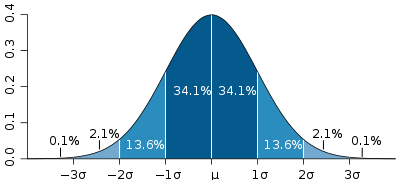
\includegraphics[scale=0.85]{regra-dos-3-sigma.png}
\label{figura:regra_3_sigmas}
\end{figure}

Após a delimitação dos valores das características de acordo com a regra do três-sigma, definimos um único formato de conjunto fuzzy para todas as variáveis do SBRF. O formato escolhido foi o triangular, por sua simplicidade, e também, pelo fato de ser muito utilizado na literatura \cite{alcala2009multiobjective, gacto2010integration, antonelli2012multi, cardenas2012multiobjective}.\todo[inline]{Inserir estas referencias: Integration of an Index to Preserve the Semantic Interpretabiliy in the MOE Rule Selection and Tuning of LFS (GACTO et al 2010), Multi-objective Evolutionary Rule and Condition Selection for Designing Fuzzy Rule-based Classifiers (Antonelli et al 2012), Alcala et al 2009 A MOEA to concurrently learn rule and data bases of linguistic FRBS, Multiobjective Genetic Generation of Fuzzy Classifiers using IRL (Cardenas e Camargo 2012) Inserir em ordem cronológica}

Para as variáveis de entrada do SBRF, nossa primeira modelagem foi dividir igualmente os dados em $2N + 1$ conjuntos fuzzy, conforme recomendado em \cite{wang1992generating}, para $N$ igual a dois, resultando em cinco regiões fuzzy: $Muito Baixo (MB)$, $Baixo (B)$, $Medio (M)$, $Alto (A)$ e $Muito Alto (MA)$. A figura \ref{figura:cinco_conjuntos_fuzzy} ilustra essa primeira modelagem.

\begin{figure}[H]
\caption{Modelagem com 5 conjuntos fuzzy}
\centering
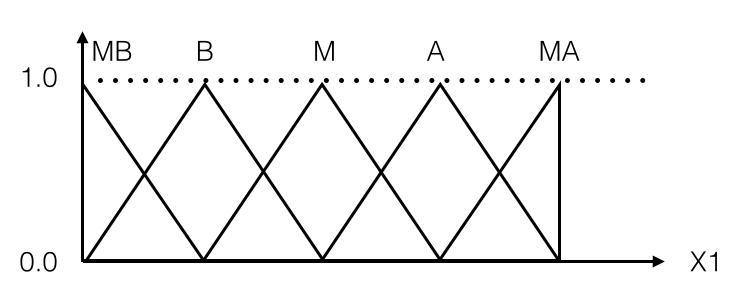
\includegraphics[scale=0.45]{cinco_conjuntos_fuzzy.png}
\label{figura:cinco_conjuntos_fuzzy}
\end{figure}

Para as variáveis de entrada do SBRF testamos três modelagens diferentes: cinco, três e dois conjuntos fuzzy, uniformemente distribuídos no domínio de cada variável. Os conjuntos fuzzy foram denominados de: $Muito Baixo (MB)$, $Baixo (B)$, $Medio (M)$, $Alto (A)$ e $Muito Alto (MA)$. A figura \ref{figura:cinco_conjuntos_fuzzy} ilustra essa primeira modelagem. As figuras \ref{figura:tres_conjuntos_fuzzy} e \ref{figura:conjuntos_fuzzy_entrada_final} ilustram as partições fuzzy com três e dois conjuntos fuzzy, respectivamente.

\begin{figure}[H]
\caption{Modelagem com 3 conjuntos fuzzy}
\centering
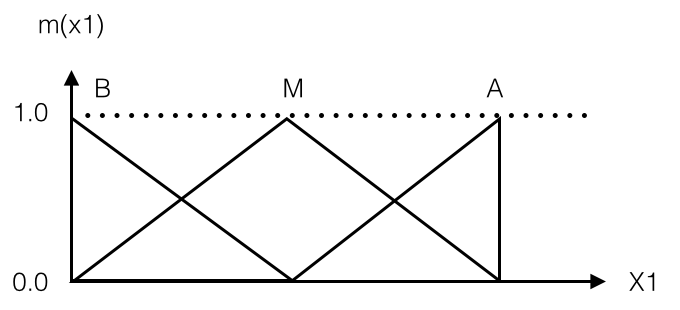
\includegraphics[scale=0.45]{tres_conjuntos_fuzzy.png}
\label{figura:tres_conjuntos_fuzzy}
\end{figure}

\begin{figure}[H]
\caption{Modelagem com 2 conjuntos fuzzy}
\centering
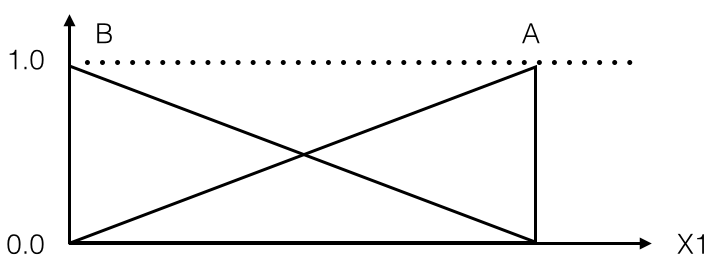
\includegraphics[scale=0.45]{conjuntos_fuzzy_entrada_final.png}
\label{figura:conjuntos_fuzzy_entrada_final}
\end{figure}

\todo[inline]{Matheus, na figura, retire o m(x1), pois isso representa o grau de pertinencia de x1 no conjunto m. Mas como o objetivo eh apenas ilustrar a particao fuzzy da variavel linguistica X1, ele nao serah necessario. Faca isso nas outras figuras tambem!}

Para a variável de saída, nós utilizamos dois conjuntos fuzzy, $Positivo (P)$ e $Negativo (N)$, distribuídos uniformemente. Isto porque, a nossa principal tarefa é classificar o sentimento geral dos documentos em positivo ou negativo. A figura \ref{figura:conjuntos_fuzzy_saida} mostra como ficou a modelagem da variável de saída.

\begin{figure}[H]
\caption{Modelagem da variável de saída em 2 conjuntos fuzzy}
\centering
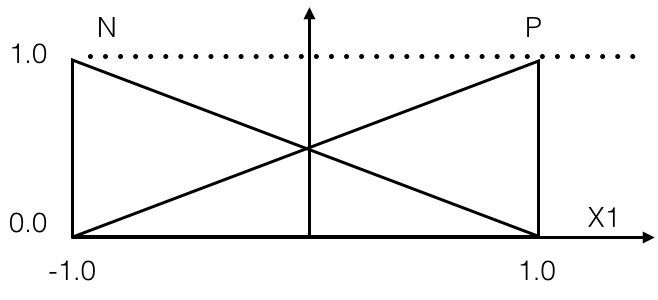
\includegraphics[scale=0.45]{conjuntos_fuzzy_saida.png}
\label{figura:conjuntos_fuzzy_saida}
\end{figure}

O uso de mais ou menos conjuntos fuzzy faz com que o mapeamento dos dados seja mais ou menos granular, possibilitando classificar casos mais específicos. Todavia, quanto maior a granularidade, mais complexo será o processo de construção das regras. Esta é uma característica do método de Wang-Mendel \cite{wang1992generating}, que foi utilizado neste trabalho, e que será detalhado na próxima seção.

\todo[inline]{Nao esquecer de explicar no capítulo de Fundamentação Teórica: granularidade, partição fuzzy. Outra coisa: as figuras não estão ficando em lugares adequados. Precisa adequar as posições delas... E tem uma figura com ??}

\subsection{O método de Wang-Mendel}

O método de Wang-Mendel é uma forma rápida para construção de regras fuzzy orientado à dados numéricos, os quais representam as amostras de um determinado conjunto de dados. A primeira etapa deste método é definir os conjuntos fuzzy das variáveis de entrada e saída. A segunda etapa é a geração das regras fuzzy a partir da combinação das variáveis de entrada e saída. A terceira etapa associa um grau para cada regra gerada. E por último, o conjunto final de regras fuzzy é gerado, eliminando as regras repetidas e inconsistentes \cite{wang1992generating}.

\todo[inline]{Matheus, vc tem duas opções: 1.Descrever de forma geral o algoritmo, ou 2.Descrever detalhadamente o algoritmo. Se vc escolher 1. Eu recomendaria tirar toda definição formal de vetor de característica, de conjunto, etc., e deixar somente texto para explicar o algoritmo. Eu recomendaria a inserção de um pseudocodigo, após o texto explicativo. Se vc escolher 2. Vc deve fazer como está no artigo, ou seja, definir formalmente como estão os seus dados (vetores de características), mostrar a partição fuzzy das varíaveis, etc... em outras palavras, seria transcrever o exemplo do artigo de Wang-Mendel. O seu texto está entre as opções 1 e 2. A opção 1 é mais simples, vc teria menos trabalho. A opção 2, vc teria que melhorar mais a sua explicação. E ai? qual vai ser?}

Uma vez definidas as regiões fuzzy (ou conjuntos fuzzy) dos dados de entrada e saída, a próxima tarefa é a criação do conjunto de regras baseadas nas características. Nosso conjunto de características pode ser representado da seguinte forma:

\begin{equation}
( x_1^1, x_2^1, ... , x_n^1, y^1), ( x_1^2, x_2^2, ... , x_n^2, y^2), ...
\label{eq:repr_feat}
\end{equation}

onde, $x_1^k, x_2^k, ... , x_n^k$ são os vetores de características e $y^k$ é a polaridade, positiva ou negativa, de um documento. Para gerar regras fuzzy a partir das  características, precisamos determinar os graus de pertinência de cada característica $x_i^k$ e $y^k$ para cada conjunto fuzzy que definimos anteriormente. Por exemplo, é preciso saber qual o grau de pertinência de $x_1^1$ para o conjunto $Alto$ e para o conjunto $Baixo$, assim como para $x_1^2$ e o grau de pertinência de $y^1$ e $y^2$ para os conjuntos $Positivo$ e $Negativo$. Em seguida, associa-se cada $x_i^k$ e $y^k$ ao conjunto fuzzy com maior grau de pertinência resultante (se $x_1^1$ teve maior grau de pertinência no conjunto $Baixo$, ele será associado a essa região, e assim sucessivamente). Assim, podemos definir a criação de uma regra fuzzy da seguinte forma:

\begin{equation}
\begin{split}
( x_1^k, x_2^k, ... , x_n^k, y^k) => [x_1^k (Pol(x_1^k) \, em \, CFI_n, max), \, ... \, , x_n^k (Pol(x_2^k) \, em \, CFI_m, max); \\
y^k(Pol(y^k) \, em \, CFS_n, max)] => Regra \, k: \\ IF \, x_1^k \, is \, CFI_n \, and \, ... \, x_n^k \, is \, CFI_m, \, THEN \, y^k \, is \, CFS_n
\label{eq:repr_fuzzy_rule}
\end{split}
\end{equation}

onde $(Pol(x_1^k) \, em \, CFI_n, max)$ é o grau máximo de pertinência alcançado por $x_1^k$ em um dos conjuntos fuzzy de entrada $CFI_n$ e $(Pol(y^k) \, em \, CFS_n, max)$ é o grau máximo de pertinência alcançado por $y^k$ um um dos conjuntos fuzzy de saída $CFS_n$. As regras geradas são do tipo "AND", que são regras em que as condições antecedentes, a parte do IF, tem de, simultaneamente ocorrer em ordem para que o conseqüente, a parte THEN, aconteça. 

A tarefa de geração de regras cria uma regra para cada vetor de característica. Devido a grande quantidade de vetores de características, é muito provável que regras conflitantes tenham sido geradas, como regras com mesmo antecedente, mas com conseqüente diferente. Uma maneira proposta pelo método de Wang-Mendel é associar um grau a cada regra e descartando a regra conflitante com menor grau. Além de eliminar regras contraditórias, esse método também reduz a quantidade de regras a serem usadas na classificação. A seguinte estratégia é utilizada para associar um grau $D(regra)$ a cada regra: 

\begin{equation}
D(regra) = m_{CFI_n}(x_1) \cdot m_{CFI_m}(x_2) \cdot m_{CFI_o}(x_n) \cdot ... \cdot m_{CFS_n}(y)
\label{eq:grau_regra}
\end{equation}

onde $m_{CFI_o}(x_n)$, por exemplo, é o grau de pertinência de $x_n$ no conjunto fuzzy $CFI_o$. Por exemplo, considere uma regra com duas características: "IF $x_1$ is Alto and $x_2$ is Alto, THEN $y$ is Positivo". O grau dessa regra, utilizando a estratégia \ref{eq:grau_regra}, é obtido assim:  $D(regra) = m_{Alto}(x_1) \cdot m_{Alto}(x_2) \cdot m_{Positivo}(y)$. Depois de eliminadas as regras conflitantes, as regras finais constituem o conjunto de regras fuzzy baseado nas características dos documentos. Com esse conjunto de regras é possível classificar os documentos da base de dados.

\subsection{Raciocínio Fuzzy}

Após a modelagem fuzzy das variáveis de entrada e saída do sistema, e da construção das regras fuzzy, é necessário definir um mecanismo de inferência fuzzy, que será responsável em determinar a polaridade (positiva ou negativa) dos documentos da base de dados. Nós utilizamos dois mecanismos para fins de comparação, o Método de Raciocínio Fuzzy Geral (MRFG) e o Método de Raciocínio Fuzzy Clássico (MCRF) \cite{cordon1999proposal}.

\todo[inline]{Eu mudei os nomes dos métodos para: Método de Raciocínio Fuzzy Geral (MRFG), Método de Raciocínio Fuzzy Clássico (MRFC), consequentemente, isso afetará as legendas de figuras, tabelas e texto :(}

Ambos mecanismos tem processos bastante similares e somente diferem na etapa de decisão na classificação. O mecanismo comum a ambos é: cada vetor de característica é avaliado por todas as regras fuzzy e um grau de compatibilidade \ref{eq:compat_regra} é calculado para cada regra. 

\todo[inline]{Quando for referenciar tabela, figura, equação, faça de forma direta. Exemplo: De acordo com a Equação 3.6, um grau de compatibilidade é calculado entre a regra i e a amostra j. A equação 3.6 deverá estar de acordo com a formalização que será apresentada na Fundamentação Teórica, ou seja, quando for descrever sobre as conjuntos fuzzy, funções de pertinência, etc.}

\begin{equation}
D(regra) = m_{CFI_n}(x_1) \cdot m_{CFI_m}(x_2) \cdot m_{CFI_o}(x_3) \cdot ...\cdot m_{CFI_p}(x_n)
\label{eq:compat_regra}
\end{equation}

O MRFC escolhe a regra que ficou com o maior grau de compatibilidade após a avaliação das características e classifica o documento com a classe de saída dessa regra. \todo[inline]{Aqui tem um erro: o metodo calcula o grau de compatibilidade da regra i com todos os padroes j. Assim, a regra terá como saída, a saída do padrão com maior compatibilidade} Por outro lado, o MRFG considera o máximo grau médio de compatibilidade entre as duas classes possíveis, positivo e negativo. Em outras palavras, o MGRF calcula a média dos graus de compatibilidade entre as regras que tem o consequente com a classe positiva e negativa e classifica o documento com a classe de maior média resultante. 

\section{Métricas de Avaliação}

A avaliação dos resultados deste trabalho foi feita usando validação cruzada de 10 dobras \todo[inline]{huuumm... dobras ficou esquisito... melhor usar folds mesmo. E accuracy pode ser acurácia.} As medidas para avaliar o desempenho da classificação do sistema foram a \textit{accuracy}, taxa real de positivos (TPR) e taxa real de negativos (TNR). A \textit{accuracy} \ref{eq:acccuracy} é uma medida da razão entre a soma dos documentos positivos (TP) e negativos (TN) corretamente classificados e o total de documentos classificados, sejam eles corretos ou não.\todo[inline]{aqui a divisão é feita pela quantidade total de documentos da base, ou seja, estes não foram classificados. Retire a parte de classificados, sejam eles corretos ou não}

\begin{equation}
Accuracy =  (TP + TN) / Total
\label{eq:acccuracy}
\end{equation}

\todo[inline]{A tradução correta é: Taxa de verdadeiro positivo, verdadeiro negativo, falso positivo e falso negativo}

A taxa real de positivos (TPR) mede a proporção de documentos positivos que são corretamente classificados como tal. Mais especificamente, a TPR mede a razão entre os documentos classificados como positivo sobre o universo de documentos realmente positivos (TP) e documentos positivos que foram classificados como negativos, conhecidos como falsos negativos (FN). A equação \ref{eq:tpr} ilustra como é feito o cálculo dessa medida. 

\begin{equation}
TPR = TP / (TP + FN)
\label{eq:tpr}
\end{equation}

A taxa real de negativos (TNR), por outro lado, mede a proporção de documentos negativos que são corretamente classificados como tal. Mais especificamente, a TNR mede a razão entre os documentos classificados como negativo sobre o universo de documentos realmente negativos (TN) e documentos negativos que foram classificados como positivos, conhecidos como falsos positivos (FP). A equação \ref{eq:tnr} ilustra como é feito o cálculo dessa medida. 

\begin{equation}
TNR = TN / (TN + FP)
\label{eq:tnr}
\end{equation}

\todo[inline]{De onde tirou as definições de TPR e TNR? No artigo de García-Pedrajas and Pérez-Rodríguez (2012) Multi-selection of instances: A straightforward way to improve evolutionary instance selection, Applied Soft Computing 12 (2012) 3590–3602. TPR é chamado de sensitivity e TNR é chamado de specificity}

Além disso, com o objetivo de verificar se as diferenças entre os resultados dos experimentos são significativas ou não, nós utilizamos o teste de \textit{Wilcoxon signed-rank} \cite{wilcoxon1945individual}, usado para comparar resultados entre conjuntos de testes relacionados, resultados sucessivos sobre um único conjunto de teste, dentre outros. Por fim, também usamos um terceiro método, o \textit{Support Vector Machine} (SVM), bastante utilizado em trabalhos de mineração de opinião dependentes de domínio e que, comumente, produz bons resultados \cite{ohana2009sentiment, moraes2012document}. Assim, podemos verificar como nossa proposta se comporta frente aos métodos tradicionais utilizados nessa área. 

\todo[inline]{SVM não é um classificador??? Aqui vc está dizendo que é um método estatístico?!}